\documentclass[../main.tex]{subfiles}
\graphicspath{{\subfix{../IMAGES/}}}

\begin{document}
\localtableofcontents

\subsection{Introduction}
EMC deals with interference and the prevention of it.\\
\begin{itemize}
    \item \textbf{Electromagnetic Disturbance (EMD) :} any electromagnetic phenomenon which may degrade the performance of a device
    \item \textbf{Electromagnetic Interference (EMI) :} degradation of the performance of a device caused by an EMD
    \item \textbf{Electromagnetic Susceptibility (to a disturbance) :} inability of a device to perform without degradation (Susceptibility is a lack of immunity.
\end{itemize}

A system is electromagnetically compatible with its environment if it satisfies 3 criteria : it does not cause interference with other systems, it is not susceptible to emission from other systems, it does not cause interference with itself.\\

3 ways to prevent interferences : suppress the emission at its source, make the coupling path as inefficient as possible, make the receptor less susceptible.\\

\quad \underline{Categories of EMC problems :}\\
Radiated emissions : cables can act as antennas; we are looking at the electromagnetic fields generated.\\
Radiated susceptibility : cables can act as antennas and pick up interferences; we are looking at the received EF.\\
Conducted emissions : a noisy source in the system injects interferences/harmonics in the system.\\
Conducted susceptibility : opposite.\\

\quad \underline{Types of sources in EMC :}\\
Natural sources : lightning, electrostatic discharge, solar \& cosmic noise ...\\
Man-made sources : electric power system noise, computer clock, switching power supplies, electric motors, nuclear EM pulse ...\\

\quad \underline{Types of signal :}\\
Narrow-band, or continuous wave (CW) spectra. Transients, large-amplitude signals (lightning \& NEMP) and weak signals (radio signals, microcircuitry ...)\\

The relationship between the frequency spectral content $F(w)$ and the transient waveform $f(t)$ is given by the Fourier transform : $F(w) = \int_{-\infty}^\infty f(t) \exp(-j\omega t)dt$, $f(t) = \frac{1}{2\pi} \int_{-\infty}^\infty F(w) \exp{j\omega t}d\omega$.\\

Many different types of EMD on an electrical system (going from least to most power level of EMD) : temporary EMI (noise in analog systems or recoverable upset in digital systems), permanent loss of function of the system (permanent upset, requiring manual intervention), equipment damage due to component failure. \\

Two different classes of digital equipment are defined : class A (devices operating in a commercial, industrial or business environment), class B (devices operating in a residential environment, more stringent than class A).\\

Limitations on EM interference are specified through conducted and radiated emissions.\\

Primary quantities of interest are : conducted emissions voltage (V) and current (A), radiated emissions E-field (V/m) and H-field (A/m). Decibels are the logarithmic ratio of two quantities : $r = 10\log_{10}(\frac{P_1}{P_2}) = 10\log_{10}(\frac{V_1^2/R}{V_2^2/R}) = 20\log_{10}(\frac{V_1}{V_2})$.\\
Absolute power, voltage or current is expressed in dB by referencing to some base quantity (voltage are expressed relative to $1\mu V$ : $U_1(dB\mu V) = 20\log_{10} \frac{U_1(V)}{1\mu V} 20 \log_{10} U_1(\mu V)$). For instance : $X(dBy) = 20\log_{10} \lfloor X(y)\rfloor$. \begin{table}[hbt!]
    \centering
    \begin{tabular}{c|c|c}
        Quantity & Unit & Ref. value \\ \hline
        Voltage & $dB\mu V$ & $1\mu V$\\
        Current & $dB\mu A$ & $1\mu A$\\
        Power & $dBmW$ & $1mW$\\
        E-field & $dB\mu V/m$ & $1\mu V/m$\\
        H-field & $dB\mu A/m$ & $1\mu A/m$\\
    \end{tabular}
\end{table}

\subsection{Coupling modes}
Electromagnetic interaction between an EMI source and a system can be classified in terms of the propagation coupling path : \textbf{conductive coupling} : propagation of V and A along conductors, \textbf{EM coupling} : propagation of EMF in a nonconductor medium/in a conductor (metallic shield). 

Analysis methods : \begin{table}[hbt!]
    \centering
    \begin{tabular}{p{.3\textwidth}|p{.3\textwidth}|p{.3\textwidth}}
         & Validity & Remarks \\ \hline
        Quasistatic & Overall dimensions $<<\lambda$min & Lumped elements, kirchhoff's model, absence of any geometrical space, analytical solution possible\\ \hline
        Transmission line (TL) & transverse dimensions $<<\lambda$min & Longitudinal propagation, distributed elements, rarely analytical solution\\ \hline
        Maxwell's equations & macroscopic scale & numerical solution needed\\
    \end{tabular}
\end{table}

\begin{figure}[hbt!]
    \centering
    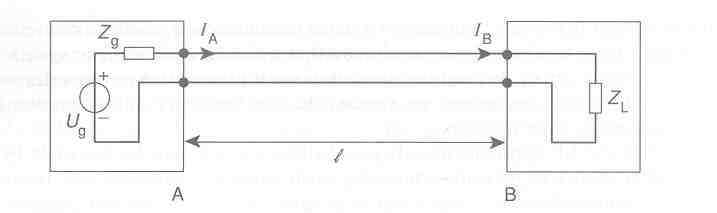
\includegraphics[width=0.5\linewidth]{IMAGES/Electromag/TLline.jpg}
\end{figure}

With the quasi-static approximation : $\lvert \frac{I_A}{I_B}\rvert = 1$.\\
TL theory : $\lvert \frac{I_A}{I_B}\rvert = \sqrt{\cos^2 kl + (\frac{Z_L}{Z_0} \sin kl)^2}$, $k=\frac{2\pi}{\lambda}$.\\


\begin{figure}[hbt!]
    \centering
    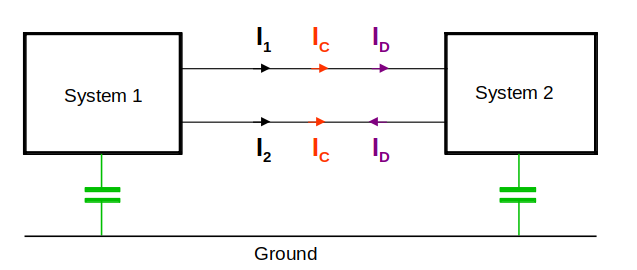
\includegraphics[width=0.5\linewidth]{IMAGES/Electromag/Screenshot from 2025-02-20 19-22-36.png}
\end{figure}
One of the most important topic affecting the radiated emissions of products is the common-mode/differential-mode currents. Differential-mode (DM) currents are equal in magnitude but oppositely directed in the wires (these are desired). The common-mode currents are equal and in the same direction (not intended!). $I_1 = I_C+I_D$, $I_2 = I_C-I_D$, $I_D = \frac{I_1-I_2}{2}$, $I_C = \frac{I_1+I_2}{2}$. \\
The radiated E-field of each current can be superimposed (a small CM current can produce the same level of radiated field as a much larger value of DM current). \\
\warning To measure $I_C$ : use a current meter that encompasses the two wires and measure $2I_C$. To get $2I_D$, use a current meter and set one wire in the opposite direction as the other.\\


Consider two simple antennas : small electric dipole and magnetic dipole.\\
$k = \frac{2\pi}{\lambda} = \frac{2\pi f}{c}$, $Z_0 = \sqrt{\frac{\mu}{\varepsilon}}$. In free-space : $Z_0 = 377\Omega$\\
\begin{itemize}
    \item Small electric dipole (of length $l$) : $E_r = \frac{Z_0}{2\pi} \frac{I_0 l \cos \theta}{r^2} (1+\frac{1}{jkr}) e^{-jkr}$, $E_\theta = \frac{j Z_0k}{4\pi} \frac{I_0 l\sin \theta}{r} (1+\frac{1}{jkr} - \frac{1}{(kr)^2}) e^{-jkr}$, $H_\phi = \frac{jk}{4\pi} \frac{I_0 l \sin \theta}{r} (1+\frac{1}{jkr}) e^{-jkr}$
    \item Small magnetic dipole (small loop with radius R and current $I_0$): $H_r = \frac{jk}{2^pi} \frac{\pi R^2 I_0 \cos \theta}{r^2} (1+\frac{1}{jkr}) e^{-jkr}$, $H_\theta = -\frac{k^2}{4\pi} \frac{\pi R^2 I_0 \sin \theta}{r} (1+\frac{1}{jkr} - \frac{1}{(kr)^2}) e^{-jkr}$, $E_\phi = \frac{Z_0 k^2}{4\pi} \frac{\pi R^2 I_0 \sin \theta}{r} (1+\frac{1}{jkr}) e^{-jkr}$.
\end{itemize}

\begin{table}[hbt!]
    \centering
    \begin{tabular}{p{.3\textwidth}|p{.3\textwidth}|p{.3\textwidth}}
         & Far fields ($kr>>1$, $\theta = 90^\circ$) & Near fields (kr<<1) \\ \hline
        Small electric dipole & $E_r = 0$, $E_\theta = \frac{jZ_0 k}{4\pi} \frac{I_0 l}{r} e^{-jkr}$, $H_\phi = \frac{jk}{4\pi} \frac{I_0l}{r} e^{-jkr}$ (wave impedance : $Z_w = \lvert \frac{E_\theta}{H_\phi}\rvert = Z_0$) & $E_r = \frac{Z_0}{2\pi jk} \frac{I_0 l \cos \theta}{r^3} e^{-jkr}$, $E_\theta = -\frac{jZ_0}{4\pi k} \frac{I_0 l \sin \theta}{r^3} e^{-jkr}$, $H_\phi = \frac{1}{4\pi} \frac{I_0 l \sin \theta}{r^2} e^{-jkr}$ (wave impedance : $Z_w = \lvert \frac{E_\theta}{H_\phi}\rvert = \frac{Z_0}{kr}$) \\ \hline
        Small magnetic dipole & $H_r = 0$, $H_\theta = -\frac{k^2}{4\pi} \frac{\pi R^2 I_0}{r} e^{-jkr}$, $E_\phi = \frac{Z_0 k^2}{4\pi} \frac{\pi R^2 I_0}{r} e^{-jkr}$ (wave impedance : $Z_w = \lvert \frac{E_\phi}{H_\theta}\rvert = Z_0$) & $H_r = \frac{1}{2\pi} \frac{\pi R^2 I_0 \cos \theta}{r^3} e^{-jkr}$, $H_\theta = \frac{1}{4\pi} \frac{\pi R^2 I_0 \sin \theta}{r^3} e^{-jkr}$, $E_\phi = \frac{Z_0 k}{4\pi} \frac{\pi R^2 I_0 \sin \theta}{r^2} e^{-jkr}$ (wave impedance : $Z_w = \lvert \frac{E_\phi}{H_\theta}\rvert = Z_0 kr$)\\
    \end{tabular}
\end{table}
\warning In far fields, the wave impedance does not depend on the source type; it is always $Z_0 = 377\Omega$.\\

\subsubsection{Transmission line theory}
A wire above the ground act as a capacitor and is therefore equivalent to two parallel conductor. \\
\warning A ground plane can be replaced by an image of the conductor.\\

\underline{Assumptions :} propagation along axis, the sum of currents at any cross section is zero, the response of the line is quasi-TEM (EMF produced by the response of the line are in the transverse plane).\\
\underline{Limitations : }for high frequency, transverse dimensions of the line are not much smaller than the wavelength.\\
At the line terminals, the transmission line component can be omitted ($I_1 = I_a + I_t$, $I_2 = I_a - I_t$ : $I_1-I_2 = 2 I_t \Rightarrow$ sum of current is zero).\\

\quad \underline{Two-conductor TL in the presence of an external EMF :}\\
The field in absence of the victim is called : excitation. The field generated by the system is called : scattered field. The sum of both is the total field.\\
Faraday's equation : $\int_c \Vec{E}\cdot d\Vec{l} = -j\omega \int \int_{\Delta S} \Vec{B} \cdot \Vec{i}_y dS$ which by taking the limit gives : $-\frac{d}{dx} \int_0^h E_z(x,z)dz + E_x(x,h)-E_x(x,0)dx = -j\omega \int_0^h  B_y(x,z)dz$. Perfect wires : $E_x(x,0) =0$, $E_x(x,h)=0$, $V(x) = -\int_0^h E_z(x,z)dz$ (transverse voltage). Remember : $\varphi(x) = \int_0^h B_y^s(x,z)dz = L' I(x)$.\\
\begin{equation}
    \frac{dV(x)}{dx} + j\omega L'I(x) = -j\omega \int_0^h B_y^e(x,z)dz
\end{equation}





\end{document}